\subsection{Model: Random Forest}

\subsubsection{Introduction}

Random Forest is an ensemble learning method that builds multiple Decision Trees and aggregates their outputs to make final predictions. This approach helps reduce overfitting while often improving generalization performance. In our experiments for sentiment classification, we trained Random Forest models across various text representations, including Count Vectorizer, TF-IDF, Word2Vec, and GloVe embeddings.

\subsubsection{Training Configuration}

The Random Forest training utilized the following hyperparameter search space:

\begin{itemize}
    \item \textbf{Number of Estimators} (\texttt{n\_estimators}): \{100\}
    \item \textbf{Maximum Depth} (\texttt{max\_depth}): \{10\}
    \item \textbf{Minimum Samples Split} (\texttt{min\_samples\_split}): \{2, 5\}
    \item \textbf{Minimum Samples Leaf} (\texttt{min\_samples\_leaf}): \{1, 2\}
    \item \textbf{Max Features} (\texttt{max\_features}): \{\texttt{"sqrt"}, \texttt{"log2"}\}
\end{itemize}

% Using K-Fold Cross-Validation, we identified the best hyperparameters based on performance metrics such as Accuracy, F1 score, and ROC AUC. The final chosen configuration was:

% \begin{itemize}
%     \item \textbf{Number of Estimators}: 100
%     \item \textbf{Maximum Depth}: 10
%     \item \textbf{Minimum Samples Split}: 5
%     \item \textbf{Minimum Samples Leaf}: 1
%     \item \textbf{Max Features}: \texttt{"sqrt"}
% \end{itemize}

A grid or random search was performed over these hyperparameters, employing K-Fold Cross-Validation to select the best configuration. The final chosen hyperparameters were validated on a withheld test set.

\subsubsection{Training and Evaluation Results}

We evaluated the Random Forest model under different feature extraction methods. The tables below provide a summary of the cross-validation (“Training”) and final testing metrics.

\textbf{Training Performance Metrics:}

\begin{table}[H]
    \centering
    \caption{Training Performance Metrics for Random Forest (Cross-Validation)}
    \label{tab:rf-training-metrics}
    \begin{tabular}{|l|c|c|c|c|c|}
        \hline
        \textbf{Method} & \textbf{Accuracy} & \textbf{ROC AUC} & \textbf{F1} & \textbf{Precision} & \textbf{Recall} \\ 
        \hline
        Count Vectorizer & 0.67 & 0.76 & 0.74 & 0.62 & 0.90 \\ 
        \hline
        TF-IDF & 0.66 & 0.65 & 0.73 & 0.61 & 0.90 \\ 
        \hline
        Word2Vec & 0.69 & 0.69 & 0.71 & 0.70 & 0.72 \\ 
        \hline
        GloVe & 0.67 & 0.67 & 0.69 & 0.68 & 0.70 \\ 
        \hline
    \end{tabular}
\end{table}

\textbf{Testing Performance Metrics:}

\begin{table}[H]
    \centering
    \caption{Testing Performance Metrics for Random Forest}
    \label{tab:rf-testing-metrics}
    \begin{tabular}{|l|c|c|c|c|c|}
        \hline
        \textbf{Method} & \textbf{Accuracy} & \textbf{ROC AUC} & \textbf{F1} & \textbf{Precision} & \textbf{Recall} \\ 
        \hline
        Count Vectorizer & 0.73 & 0.80 & 0.76 & 0.70 & 0.82 \\ 
        \hline
        TF-IDF & 0.66 & 0.75 & 0.73 & 0.62 & 0.91 \\ 
        \hline
        Word2Vec & 0.70 & 0.77 & 0.71 & 0.70 & 0.73 \\ 
        \hline
        GloVe & 0.68 & 0.75 & 0.70 & 0.68 & 0.71 \\ 
        \hline
    \end{tabular}
\end{table}

\textbf{Best Model Selection Criteria:}

\begin{itemize}
    \item The best model is chosen based on testing performance, prioritizing Accuracy > F1 Score > ROC AUC.
    \item Using this criterion, the top-performing setup is:
\end{itemize}

\begin{verbatim}
{
    "method": "count",
    "model": "RandomForestClassifier",
    "hyperparameters": {
        "max_depth": 10,
        "max_features": "sqrt",
        "min_samples_leaf": 1,
        "min_samples_split": 5,
        "n_estimators": 100
    },
    "performance": {
        "accuracy": 0.7251,
        "precision": 0.6970,
        "recall": 0.8247,
        "f1": 0.7555,
        "roc_auc": 0.8039885096586928
    }
}
\end{verbatim}

\subsubsection{Performance Analysis}

\begin{itemize}
    \item \textbf{Accuracy Analysis}: The Random Forest model trained on Count Vectorizer achieved the highest testing accuracy (72.51\%), outperforming TF-IDF, Word2Vec, and GloVe.
    \item \textbf{Ensemble Strength}: By aggregating multiple Decision Trees, the model showed resilience to overfitting, maintaining solid generalization performance.
    \item \textbf{ROC AUC}: The best model reached 0.80 in ROC AUC, indicating strong discriminative ability between the sentiment classes.
    \item \textbf{Precision and Recall}: A precision of 69.70\% and recall of 82.47\% suggest a relatively balanced performance, with a slight emphasis on correctly identifying positive cases.
    \item \textbf{Embedding Effectiveness}: Similar to other classification models in our study, simple Count Vectorizer features worked effectively. Embedding-based methods performed well but did not surpass the Count Vectorizer in final testing accuracy.
\end{itemize}

\subsubsection{Visualization of Training Results}

The following figures illustrate the model’s performance across different embedding techniques:
\begin{figure}[H]
    \centering
    \begin{subfigure}[b]{0.44\textwidth}
        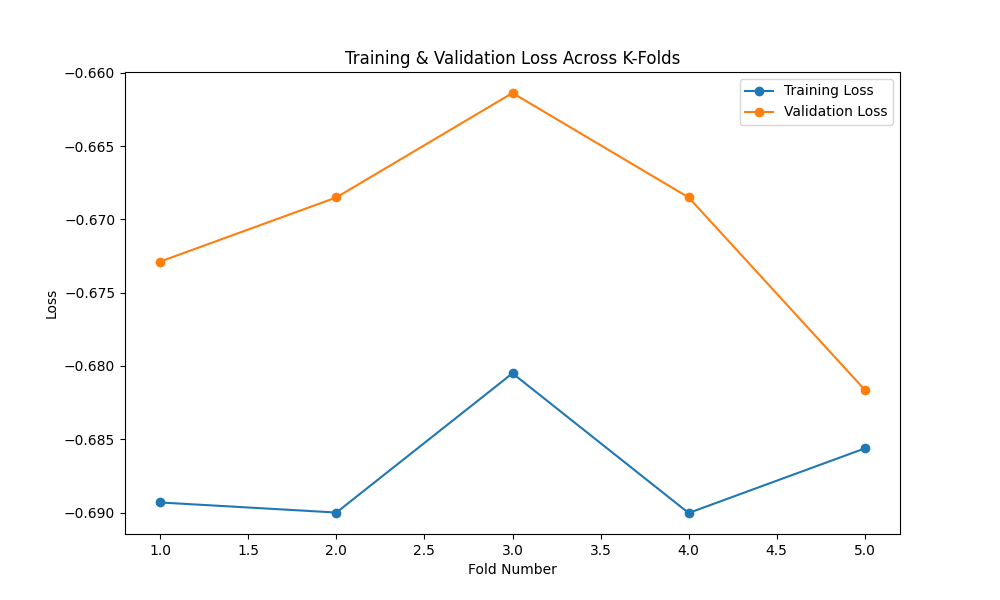
\includegraphics[width=\textwidth]{img/report_info/img/1.4.RF/best_random_forest_count_loss.png}
        \caption{Loss Curve - Count Vectorizer}
        \label{fig:rf-count-loss}
    \end{subfigure}
    \begin{subfigure}[b]{0.44\textwidth}
        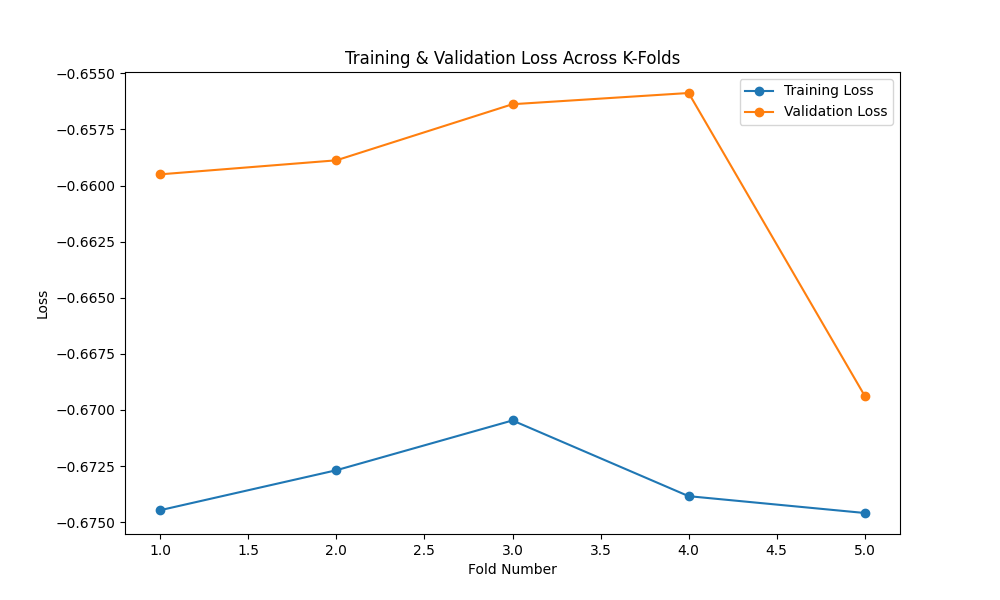
\includegraphics[width=\textwidth]{img/report_info/img/1.4.RF/best_random_forest_tfidf_loss.png}
        \caption{Loss Curve - TF-IDF}
        \label{fig:rf-tfidf-loss}
    \end{subfigure}
    
    \begin{subfigure}[b]{0.44\textwidth}
        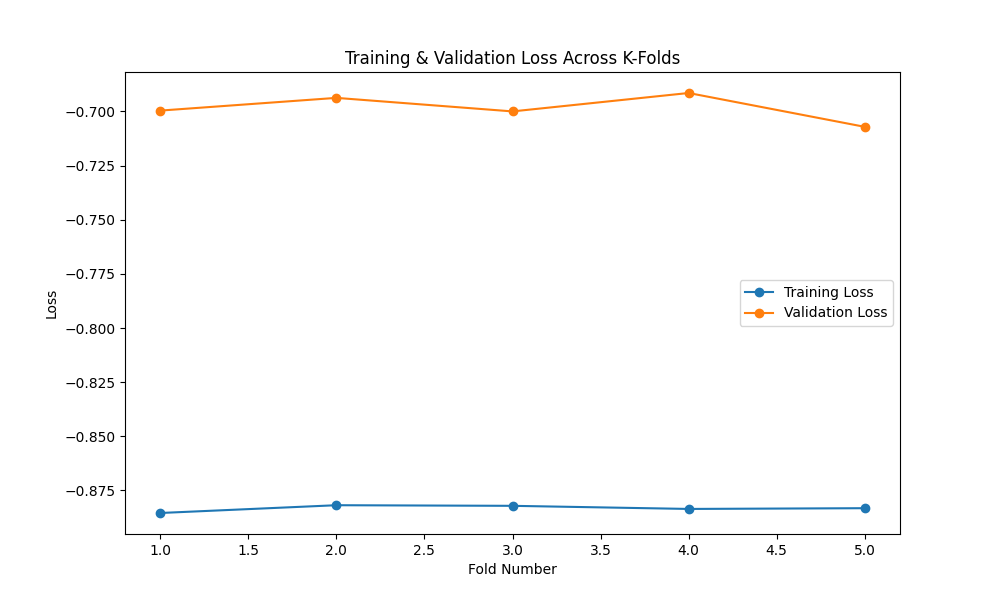
\includegraphics[width=\textwidth]{img/report_info/img/1.4.RF/best_random_forest_word2vec_loss.png}
        \caption{Loss Curve - Word2Vec}
        \label{fig:rf-word2vec-loss}
    \end{subfigure}
    \begin{subfigure}[b]{0.44\textwidth}
        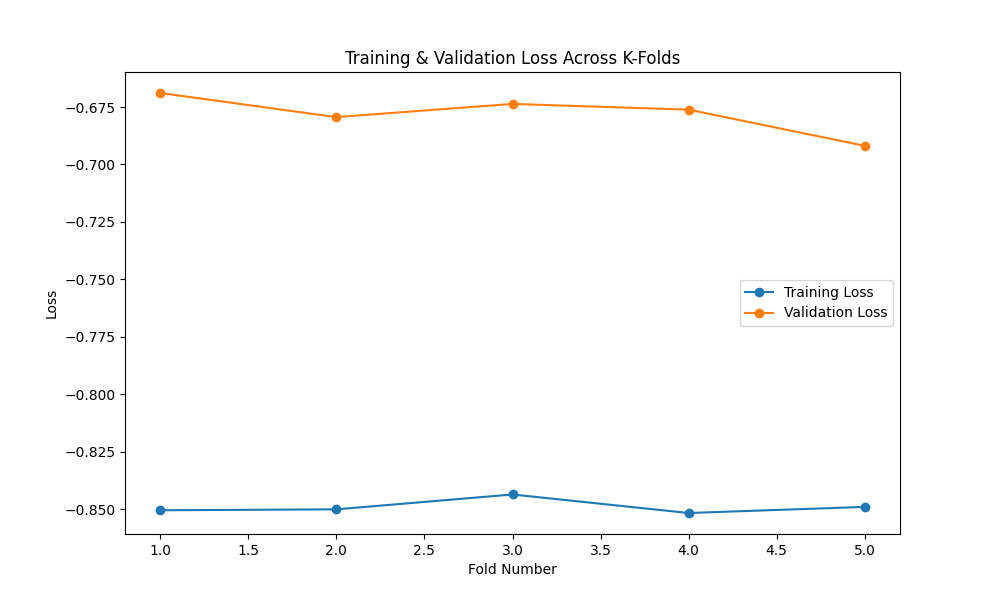
\includegraphics[width=\textwidth]{img/report_info/img/1.4.RF/best_random_forest_glove_loss.png}
        \caption{Loss Curve - GloVe}
        \label{fig:rf-glove-loss}
    \end{subfigure}
    
    \caption{Comparison of Loss Curves for Random Forest across Different Feature Extraction Methods}
    \label{fig:rf-loss-group}
\end{figure}

\begin{figure}[H]
    \centering
    \begin{subfigure}[b]{0.48\textwidth}
        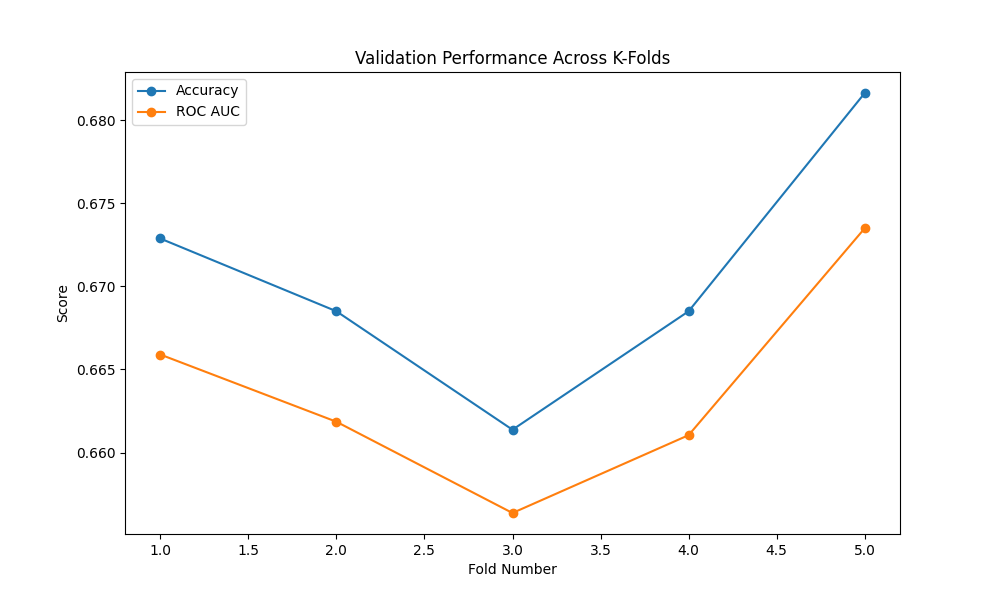
\includegraphics[width=\textwidth]{img/report_info/img/1.4.RF/best_random_forest_count.png}
        \caption{Performance - Count Vectorizer}
        \label{fig:rf-count}
    \end{subfigure}
    \begin{subfigure}[b]{0.48\textwidth}
        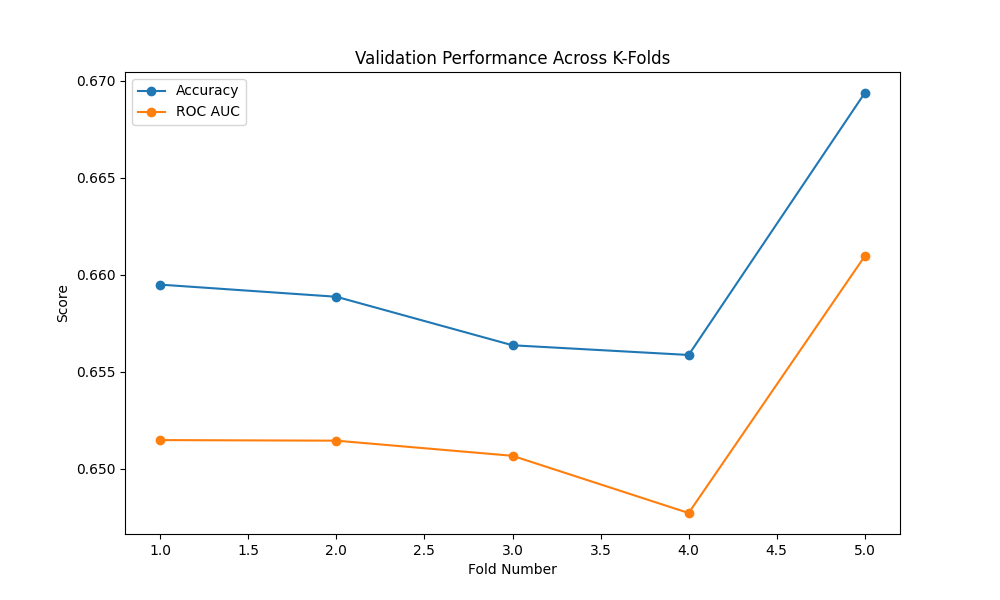
\includegraphics[width=\textwidth]{img/report_info/img/1.4.RF/best_random_forest_tfidf.png}
        \caption{Performance - TF-IDF}
        \label{fig:rf-tfidf}
    \end{subfigure}
    
    \begin{subfigure}[b]{0.48\textwidth}
        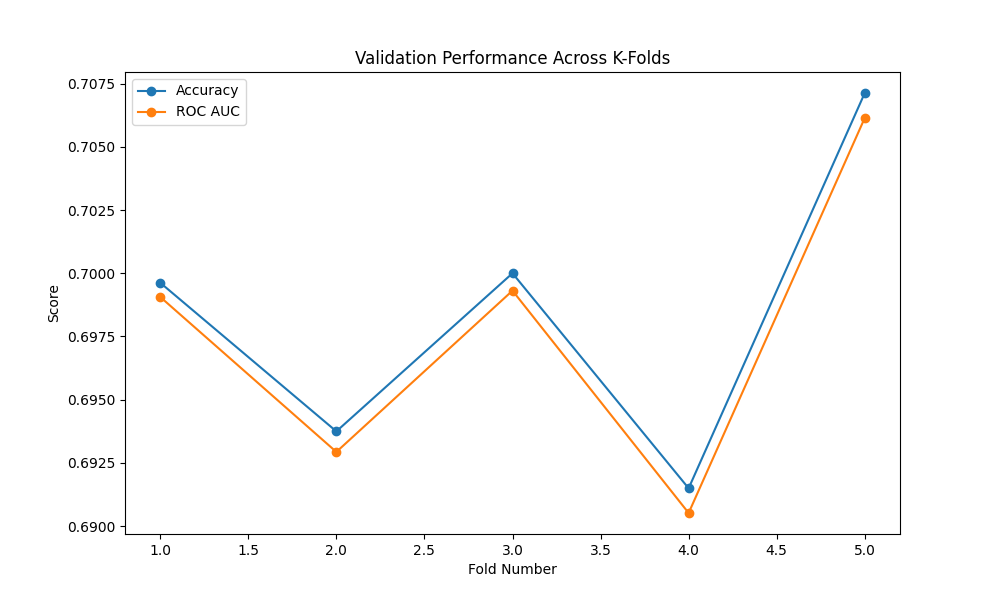
\includegraphics[width=\textwidth]{img/report_info/img/1.4.RF/best_random_forest_word2vec.png}
        \caption{Performance - Word2Vec}
        \label{fig:rf-word2vec}
    \end{subfigure}
    \begin{subfigure}[b]{0.48\textwidth}
        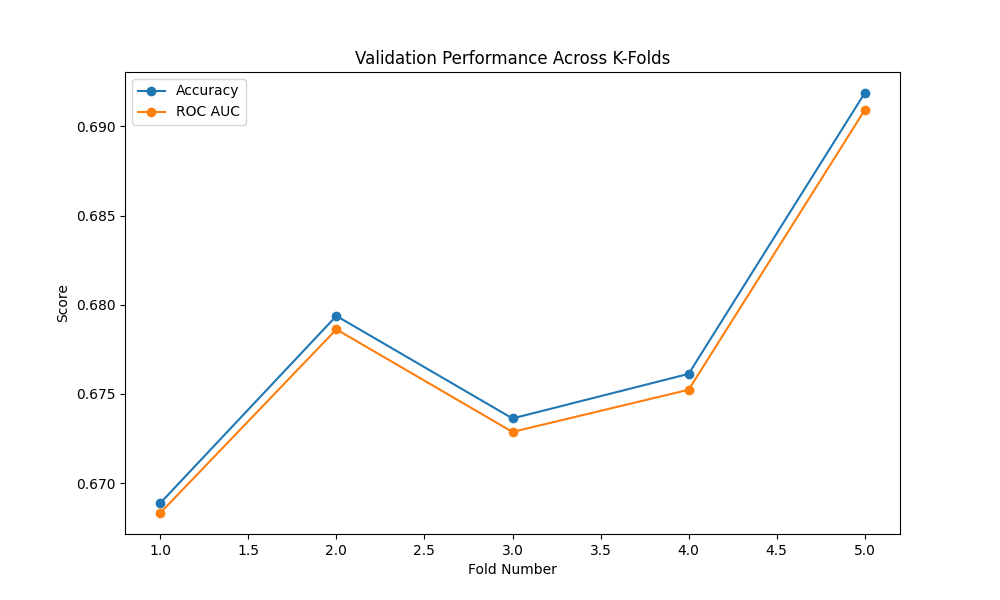
\includegraphics[width=\textwidth]{img/report_info/img/1.4.RF/best_random_forest_glove.png}
        \caption{Performance - GloVe}
        \label{fig:rf-glove}
    \end{subfigure}
    
    \caption{Comparison of Training Performance Metrics for Random Forest across Different Feature Extraction Methods}
    \label{fig:rf-performance-group}
\end{figure}

\textbf{Image Description:}

\begin{itemize}
    \item \textbf{Training and Validation Loss Analysis:}
    \begin{itemize}
        \item Overall, the Random Forest loss curves remain relatively stable across K-Fold splits.
        \item Count Vectorizer and Word2Vec often exhibit smoother convergence, while TF-IDF and GloVe may show slightly higher variance in some folds.
        \item The gap between training and validation loss is moderately low, suggesting controlled overfitting.
    \end{itemize}
    
    \item \textbf{Validation Performance Metrics:}
    \begin{itemize}
        \item Count Vectorizer achieves the highest accuracy and F1 scores in most folds, aligning with the final model selection.
        \item TF-IDF maintains decent performance but can display sharper drops in certain folds.
        \item Word2Vec offers balanced performance, though it generally trails Count Vectorizer by a small margin.
        \item GloVe tends to exhibit the most fluctuation in validation metrics, correlating with lower stability in performance.
    \end{itemize}
\end{itemize}

\subsubsection{Conclusion}

Random Forest demonstrated strong performance, with the Count Vectorizer approach delivering the highest accuracy (72.51\%) among all tested embedding methods. The ensemble nature of Random Forest mitigates overfitting risks and provides stable, competitive results in sentiment classification. Future work may explore deeper trees or larger \texttt{n\_estimators} to further enhance performance, as well as the integration of more sophisticated text representation techniques.

